\documentclass[11pt]{article}
\usepackage[utf8]{inputenc}
\usepackage[T1]{fontenc}
\usepackage{amssymb}
\usepackage{booktabs}
\usepackage{array}
\usepackage{filecontents}
\usepackage{pgfplotstable}
\usepackage{graphicx}
\pgfplotstableset{
  empty cells with={---},
  every head row/.style={before row=\toprule,after row=\midrule},
  every last row/.style={after row=\bottomrule}
}
\pgfplotsset{compat=1.9}

\begin{document}
\title{Computação Natural - TP3\\Redes Neurais}
\author{Guilherme Torres\\Departamento de Ciência da Computação - UFMG}
\date{}
\maketitle

\section{Introdução}

O objetivo do trabalho que segue é fazer uma rede de aprendizado, baseada em algum tipo de redes neurais, para montar um algoritmo que reconheça a localidade de uma proteína dentro da célula de acordo com os parâmetros que são dados. A base de dados é extremamente irregular e as redes costumam ter cerca de 60\% de acurácia.

Como modelo de rede neural, foi escolhido a rede MLP (Multi Layer Perceptron) e foi utilizada a biblioteca Keras, com backend Tensorflow. Para plotar os gráficos com os resultados dos treinos e validações, foi usado o pacote de Python matplotlib. Para executar o programa, é necessário ter esses pacotes e Python 3.5.

Os detalhes sobre as escolhas feitas no algoritmo estão explicadas a seguir.

\section{Implementação}

\subsection{O algoritmo}

Uma rede MLP é uma rede com várias camadas de perceptrons. Perceptrons são modelos de neurônios, que recebem entradas e propagam uma saída. Cada sinapse (como é chamada a conexão) do percetron é atribuída a um peso, que regula a sua influência no perceptron, e esse peso é tipicamente um número de -1 a 1.

O processo de aprendizado da rede consiste em ajustar pesos, até que, para um conjunto de entradas, a MLP consiga produzir saídas próximas das desejadas com uma acurácia desejável. Isso acontece tipicamente nas redes supervisionadas: redes onde se tem um conjunto de saídas esperadas para cada caso de treino e teste.

Esquema geral da execução do programa:

\begin{enumerate}
	\item Inicializa o algoritmo, recebendo a entrada e convertendo os dados para a rede
	\item Separa a entrada entre conjunto de treino e conjunto de validação (tipicamente uma relação 67\%-33\%)
	\item Treina a rede
	\begin{enumerate}
		\item Calcula o output final para a entrada
		\item Atualiza os pesos segundo o erro e a função de perda
		\item Faz a validação dos resultados
	\end{enumerate}
	\item Após acabar o número de iterações: recebe um histórico dos treinos e plota um gráfico segundo as gerações.
\end{enumerate}

\subsection{Parâmetros do algoritmo}

\subsection*{Função de erro}

Como estamos lidando com um problema de classificação, as backends Tensorflow e Theano oferecem uma função de perda especial para esses casos, a \textit{categorical cross entropy}. A fórmula matemática para ela pode ser encontrada nas referências [1].

Outra opção seria usar uma saída que seria um número inteiro, e considerar cada uma das categorias um número inteiro. Nesse caso, poderia ser usado um \textit{back propagation} com descida do gradiente para atualizar os pesos.

\subsection*{Neurônios nas camadas escondidas}

A quantidade de neurônios nas camadas escondidas, bem como o número delas, é um parâmetro importante de uma rede neural, porque dependendo do número de conexões que é formado, a rede pode não convergir bem, ou até, no caso de muitos, demorar muito para convergir sem que haja uma melhoria significativa no resultado.

Isso é uma decisão complicada e existem várias heurísticas (regras do dedão) para escolher esse parâmetro. Como existem 8 vias de entrada e 7 de saída (para representar as 7 categorias), assumiu-se que a soma dos dois, 15 seria um número adequado para esse parâmtro, porém isso será testado.

\subsection*{Número de camadas escondidas}

Esse parâmetro é semelhante ao outro em vários sentidos, porém sabe-se que redes de deep learning, com um intervalo maior para um treino, podem obter acurácias melhores nos seus testes. Isso também será testado.

\subsection{Outros parâmetros}

Em testes prioritários, que não serão relatados aqui (a maior parte deles não foi completa), uma última gama de padrões foi considerada antes e não houve muitos ajustes posteriores quanto a eles, por diferentes razões.

\subsection*{Inicialização dos pesos}

A inicialização dos pesos fez uma diferença insignificante na rede. As opções oferecidas pelo back-end foram distribuição normal, distribuição uniforme ou zero. A distribuição normal teve uma divergência maior de pesos no início, mas isso logo foi corrigido. Em todos os testes, foi usada a ativação normal.

\subsection*{Função de ativação}

Foi usada a função sigmóide para a ativação dos neurônios em todos os testes que possuíam até 2 camadas escondidas. Para redes mais profundas, é sabido que a ReLu agiliza o processo de aprendizado, portanto, ela foi utilizada.

\subsection*{Épocas de treinamento}

Ao longo das experimentações, concluiu-se que havia um momento a partir de cerca de 100 iterações, a partir do qual tanto os resultados para a validação quanto para o treino atingiam um \textit{plateau} e deixavam de convergir. Como foi previsto anteriormente, isso ocorre próximo aos 60\% de acurácia.

É intuitivo que as redes mais profundas levam mais tempo para convergir até atingir o seu \textit{plateau}, e devido a isso, foram usadas 150 iterações como um limite satisfatório. Isso pode não fazer a rede convergir até o seu estado final, porém a partir dos gráficos é possível reconhecer se ainda há um progresso nesse sentido.

\section{Experimentos}

Os experimentos foram realizados em um computador com sistema operacional Debian 9 unstable, 8GB de memória RAM e processador Pentium G4400 (3.3GHz). Os gráficos foram plotados usando a biblioteca matplotlib. A seguir segue a perda ao longo das iterações e a porcentagem de acurácia do modelo, avaliando-se cada um dos parâmetros.

Uma coisa comum que se observa nos experimentos, entretanto, é que pode haver, durante as fases intermediárias do treino, uma diferença grande entre os acertos no grupo de treino e no grupo de validação, chegando a cerca de 12 pontos percentuais nos piores casos. Porém, isso logo é corrigido nos experimentos que obtiveram resultados bons, fazendo com que a nova diferença no final das iterações esteja entre 4 e 2 pontos percentuais. Isso é um sinal de que, por mais que seja um problema de classificação complicado, não há muito overfitting nos casos de teste.

Sabendo disso, não foram necessárias mudanças posteriores para resolver overfitting.

\subsection*{Número de neurônios nas camadas escondidas}

Foram feitos testes com o número de neurônios iguais a 5, 10, 15 e 30. Seguem os gráficos para cada um deles (figuras de 1 a 8)

\begin{figure}
	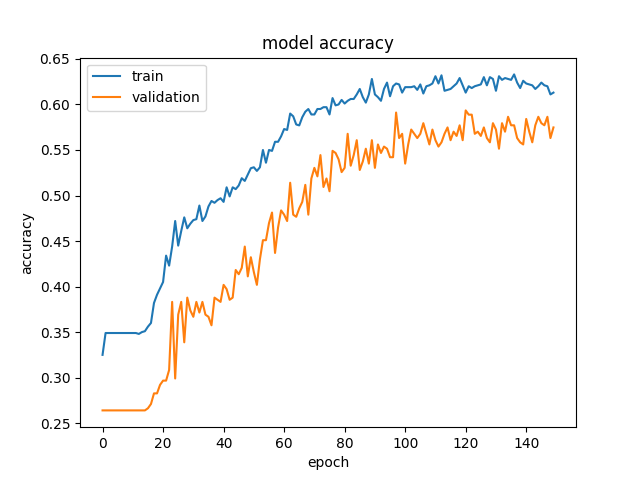
\includegraphics[width=\linewidth]{exp/Figure_1.png}
	\caption{1 camada escondida com 5 neurônios: acurácia}
	\label{fig:f1}
\end{figure}

\begin{figure}
	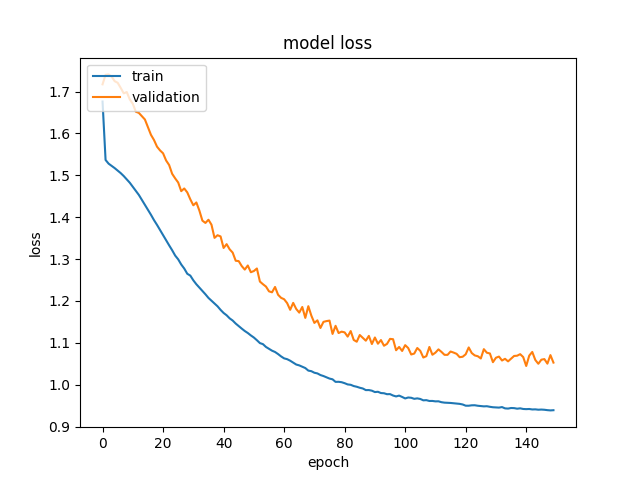
\includegraphics[width=\linewidth]{exp/Figure_1-1.png}
	\caption{1 camada escondida com 5 neurônios: perda}
	\label{fig:f11}
\end{figure}

\begin{figure}
	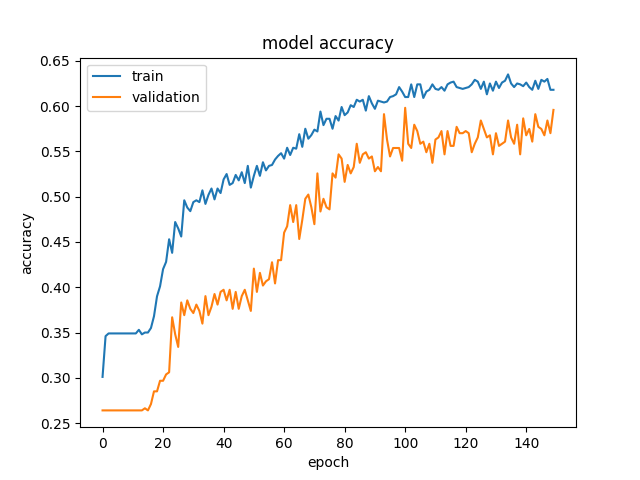
\includegraphics[width=\linewidth]{exp/Figure_2.png}
	\caption{1 camada escondida com 10 neurônios: acurácia}
	\label{fig:f2}
\end{figure}

\begin{figure}
	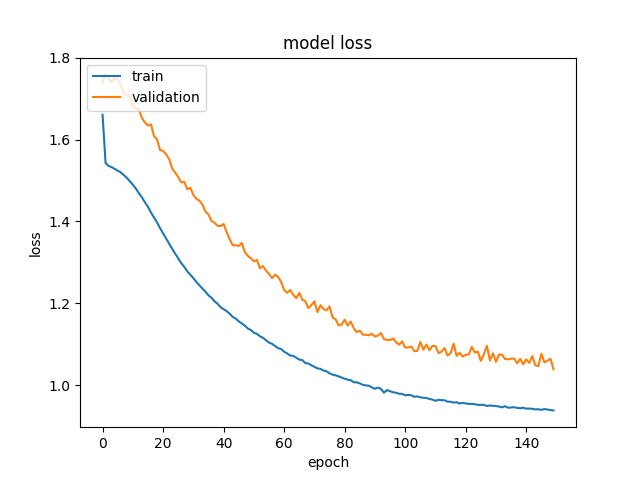
\includegraphics[width=\linewidth]{exp/Figure_2-2.png}
	\caption{1 camada escondida com 10 neurônios: perda}
	\label{fig:f21}
\end{figure}

\begin{figure}
	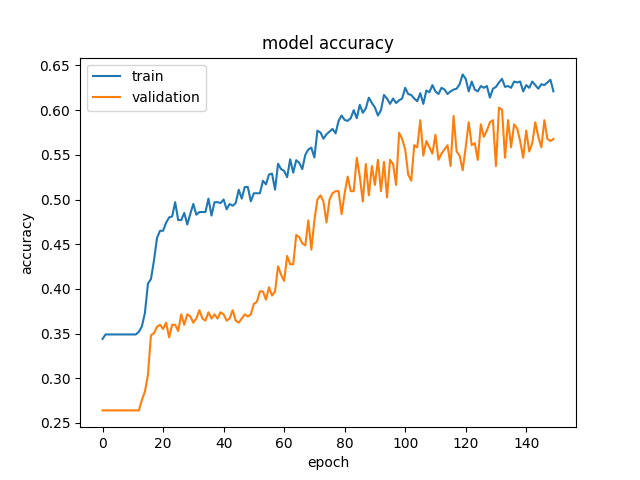
\includegraphics[width=\linewidth]{exp/Figure_3.png}
	\caption{1 camada escondida com 15 neurônios: acurácia}
	\label{fig:f3}
\end{figure}

\begin{figure}
	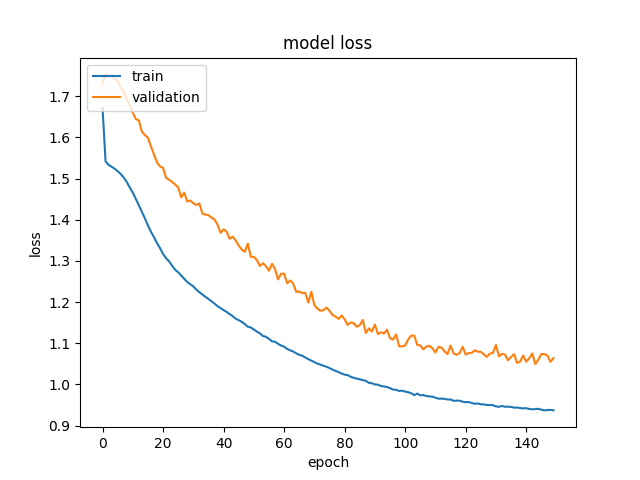
\includegraphics[width=\linewidth]{exp/Figure_3-2.png}
	\caption{1 camada escondida com 15 neurônios: perda}
	\label{fig:f31}
\end{figure}

\begin{figure}
	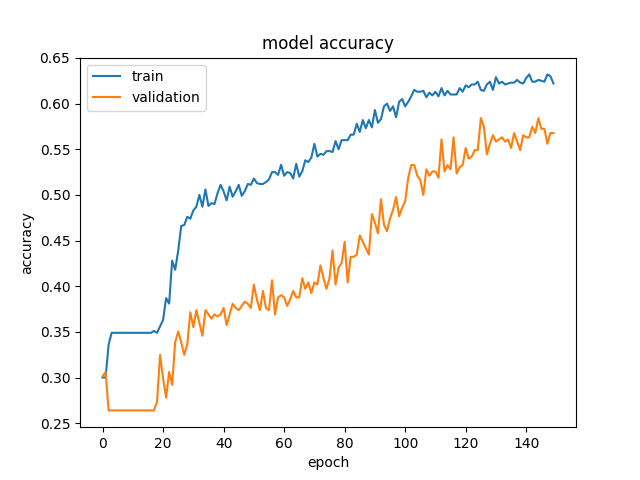
\includegraphics[width=\linewidth]{exp/Figure_4.png}
	\caption{1 camada escondida com 30 neurônios: acurácia}
	\label{fig:f4}
\end{figure}

\begin{figure}
	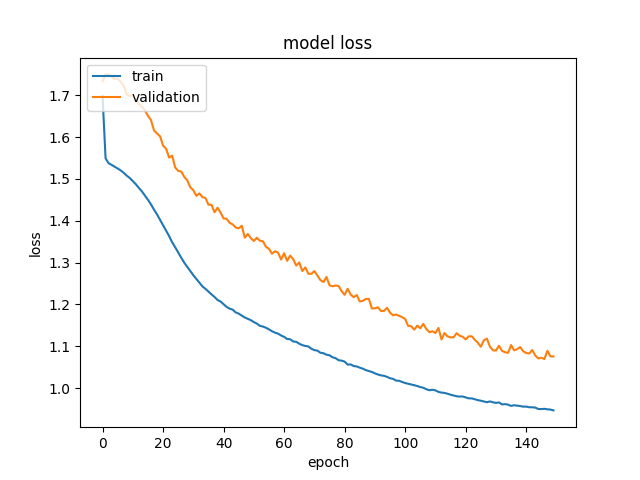
\includegraphics[width=\linewidth]{exp/Figure_4-2.png}
	\caption{1 camada escondida com 30 neurônios: perda}
	\label{fig:f41}
\end{figure}

Após analisar os gráficos, percebemos que em todos eles, os resultados para o treino são satisfatórios, porém há mudanças nos resultados para a validação. Acima de 10 camadas, os resultados para a validação são instáveis. Isso significa que, pelo menos no tempo no qual a rede foi treinada, não foi possível uma convergência para estabilizar esse conjunto. Pode-se também falar em \textit{overfitting}, nesse caso. 

Nos testes posteriores, serão usados 10 neurônios nas camadas escondidas, sendo que 5 e 10 foram os resultados mais estáveis, e 10 conseguiu chegar a taxas de perda ligeiramente menores.

\subsection*{Número de camadas escondidas}

Nas figuras de 9 a 11, segue os gráficos da acurácia dos modelos para o número de camadas escondidas. Foram usadas 2, 6 e 10 camadas, respectivamente.

\begin{figure}
	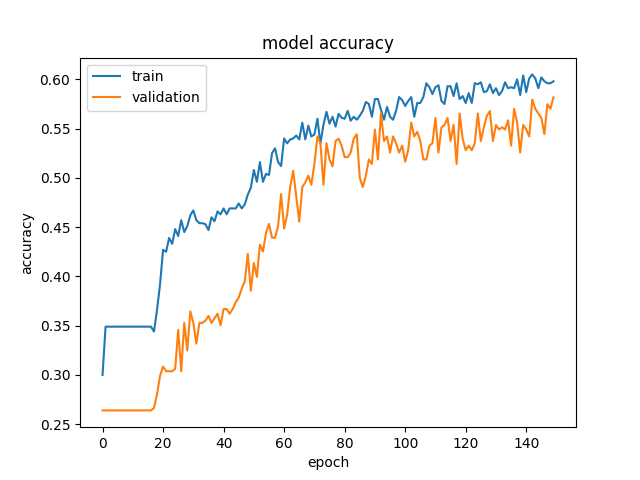
\includegraphics[width=\linewidth]{exp/Figure_5.png}
	\caption{2 camadas escondidas com 10 neurônios: acurácia}
	\label{fig:f4}
\end{figure}

\begin{figure}
	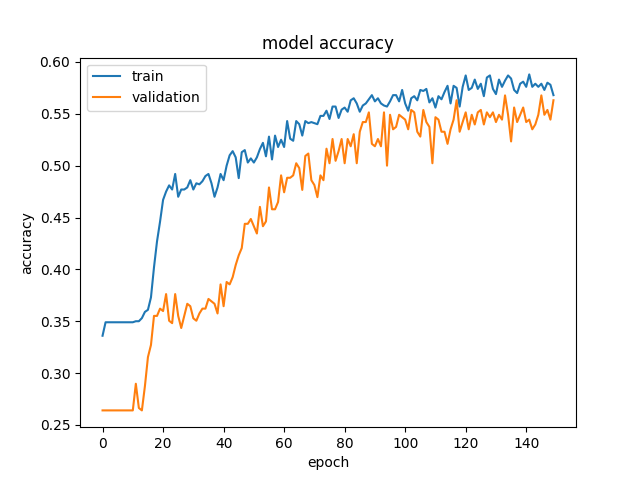
\includegraphics[width=\linewidth]{exp/Figure_6.png}
	\caption{6 camadas escondidas com 10 neurônios: acurácia}
	\label{fig:f4}
\end{figure}
\begin{figure}
	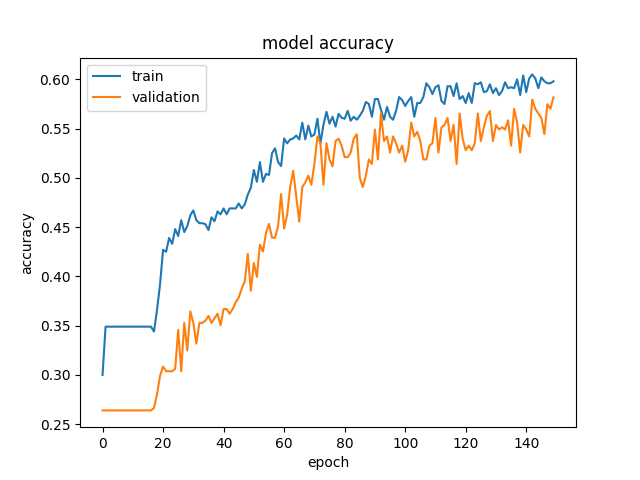
\includegraphics[width=\linewidth]{exp/Figure_5.png}
	\caption{2 camadas escondidas com 10 neurônios: acurácia}
	\label{fig:f4}
\end{figure}

\begin{figure}
	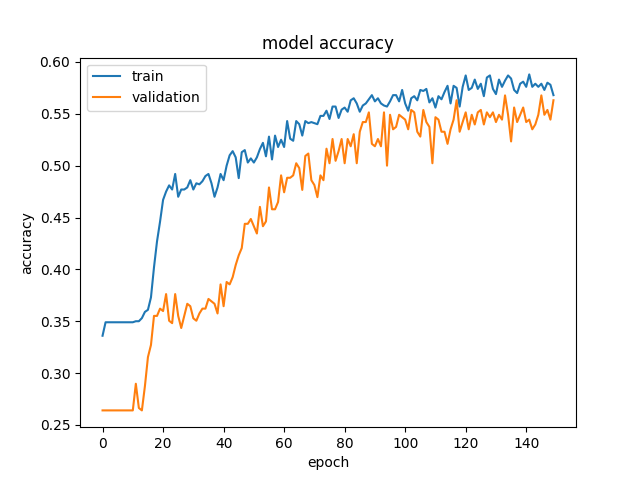
\includegraphics[width=\linewidth]{exp/Figure_6.png}
	\caption{6 camadas escondidas com 10 neurônios: acurácia}
	\label{fig:f4}
\end{figure}

\begin{figure}
	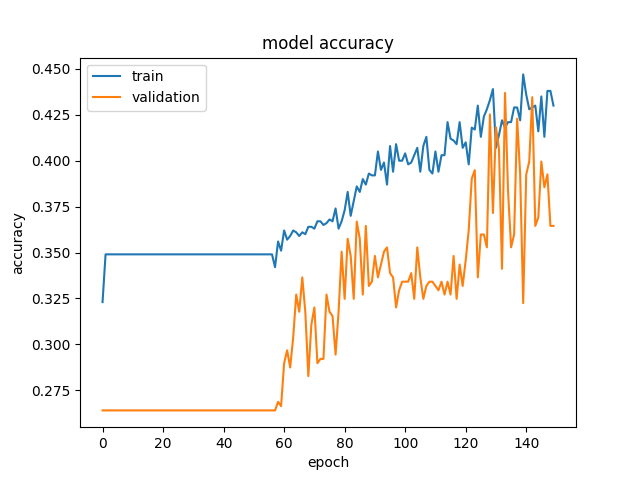
\includegraphics[width=\linewidth]{exp/Figure_7.png}
	\caption{10 camadas escondidas com 10 neurônios: acurácia}
	\label{fig:f4}
\end{figure}


Uma observação interessante sobre esses experimentos é a tendência que os resultados, à medida que o número de camadas escondidas aumenta, tendem a ficar mais instáveis e ter oscilações maiores. Isso ocorre pelo excesso de conexões que aparecem na rede: é um sinal de que ela deve ser treinada por mais gerações até que isso se estabilize. 

Porém, a partir de certo ponto, usar uma rede profunda para o problema, dependendo do tamanho do espaço de treinamento, pode ser problemático. Observamos na figura 7 que, ao usar 10 camadas escondidas, sequer há uma convergência e provavelmente não haverá. Isso também se explica pelo excesso de conexões desnecessárias.

Os experimentos com redes profundas, no geral, não só obtiveram os seus melhores resultados com menos camadas, como também não tiveram resultados melhores do que a rede com apenas uma camada escondida.

\subsection*{Mini-batches}

Sabe-se que é possível treinar a rede usando batches, que são pequenos conjuntos de exemplos que são avaliados antes de se atualizar os pesos da rede. A abordagem por mini batches é conhecida por usar menos recursos computacionais, portanto é justo que ela seja considerada nesse trabalho também. Resultados usando batches de 2, 5 e 10 seguem nos gráficos das figuras de 12 a 14. A quantidade de épocas de treinamento foi adequada ao tamanho dos mini-batches.

\begin{figure}
	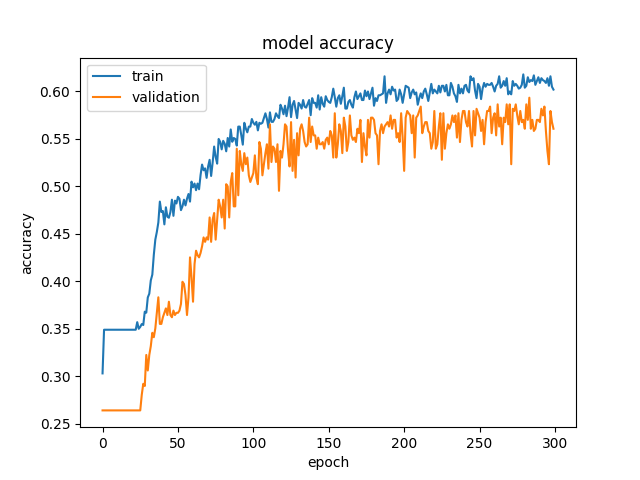
\includegraphics[width=\linewidth]{exp/Figure_8.png}
	\caption{Mini-batches de tamanho 2}
	\label{fig:f4}
\end{figure}

\begin{figure}
	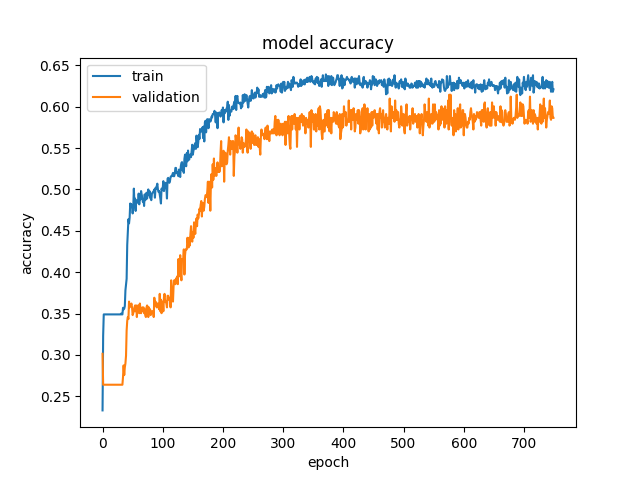
\includegraphics[width=\linewidth]{exp/Figure_9.png}
	\caption{Mini-batches de tamanho 5}
	\label{fig:f4}
\end{figure}

\begin{figure}
	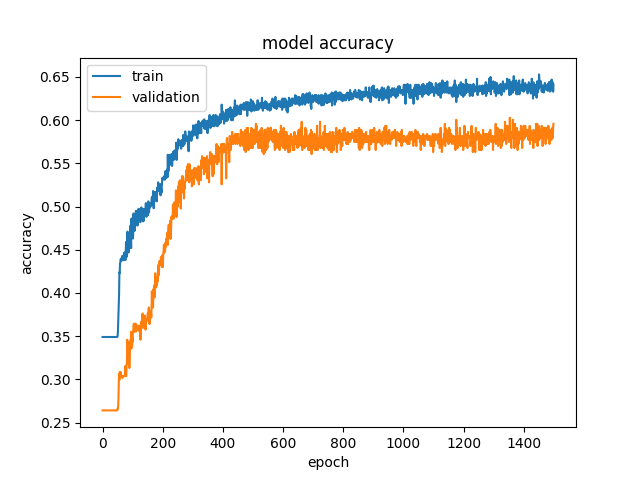
\includegraphics[width=\linewidth]{exp/Figure_10.png}
	\caption{Mini-batches de tamanho 10}
	\label{fig:f4}
\end{figure}

Os resultados, no final, chegam a níveis semelhantes aos do algoritmo sem os batches, porém o que é notável é a velocidade na qual os exemplos com batches convergiram para o seu ponto máximo. Deve-se lembrar que todos esses experimentos foram realizados na mesma escala de tempo, porém os exemplos com batches maiores chegam a convergir para o seu estado final muito mais facilmente, agilizando o processo de treino. Por exemplo, a partir dos batches de tamanho 5, como mostra a figura 9, a rede já estava atingindo resultados satisfatórios antes da metade do fim das épocas!

No caso da rede com batch size 10, já não há qualquer melhoria a partir da metade do percurso, apenas algumas oscilações, que eventualmente até pioram o resultado médio. Ou seja, não há porquê continuar treinando a rede ao se passar desse ponto.

Portanto, no caso, o uso de batches é totalmente justificável, e eles cumprem com a sua proposta de reduzir os custos computacionais.

\section{Conclusões}

Com esse trabalho, podemos tirar algumas conclusões sobre redes supervisionadas. Em primeiro lugar, atentamos ao fato de que a mesma característica que molda tantos algoritmos bioinspirados se manifesta prioritariamente em redes neurais: os parâmetros a se resolver, como quantidade de conexões, número de camadas escondidas e tamanho dos batches são definios ou experimentalmente, ou por meio de heurísticas.

Também concluímos a atenção que devemos dar ao usar uma base de dados equilibrada. A base de dados que temos em questão não é equilibrada, por há muito mais exemplos que pertencem a uma categoria do que a outra, o que influencia nas altas taxas de erro que são típicas para esse exemplo. Uma possível melhoria no trabalho seria testar usando um meio de \textit{oversampling} (multiplicação de exemplos que pertencem a uma categoria minoritária para regular a base artificialmente).

\section{Referências}

\begin{enumerate}
	\item \texttt{http://deeplearning.net/software/theano/library/tensor/nnet/nnet.html}
\end{enumerate}

\end{document}
